\section{System Architecture} \label{sec:sysarc}


The control system architecture is a relatively flat DDS message based system using multi cast messaging. A high level view is given in \figref{fig:arc}



\begin{figure}
\begin{center}
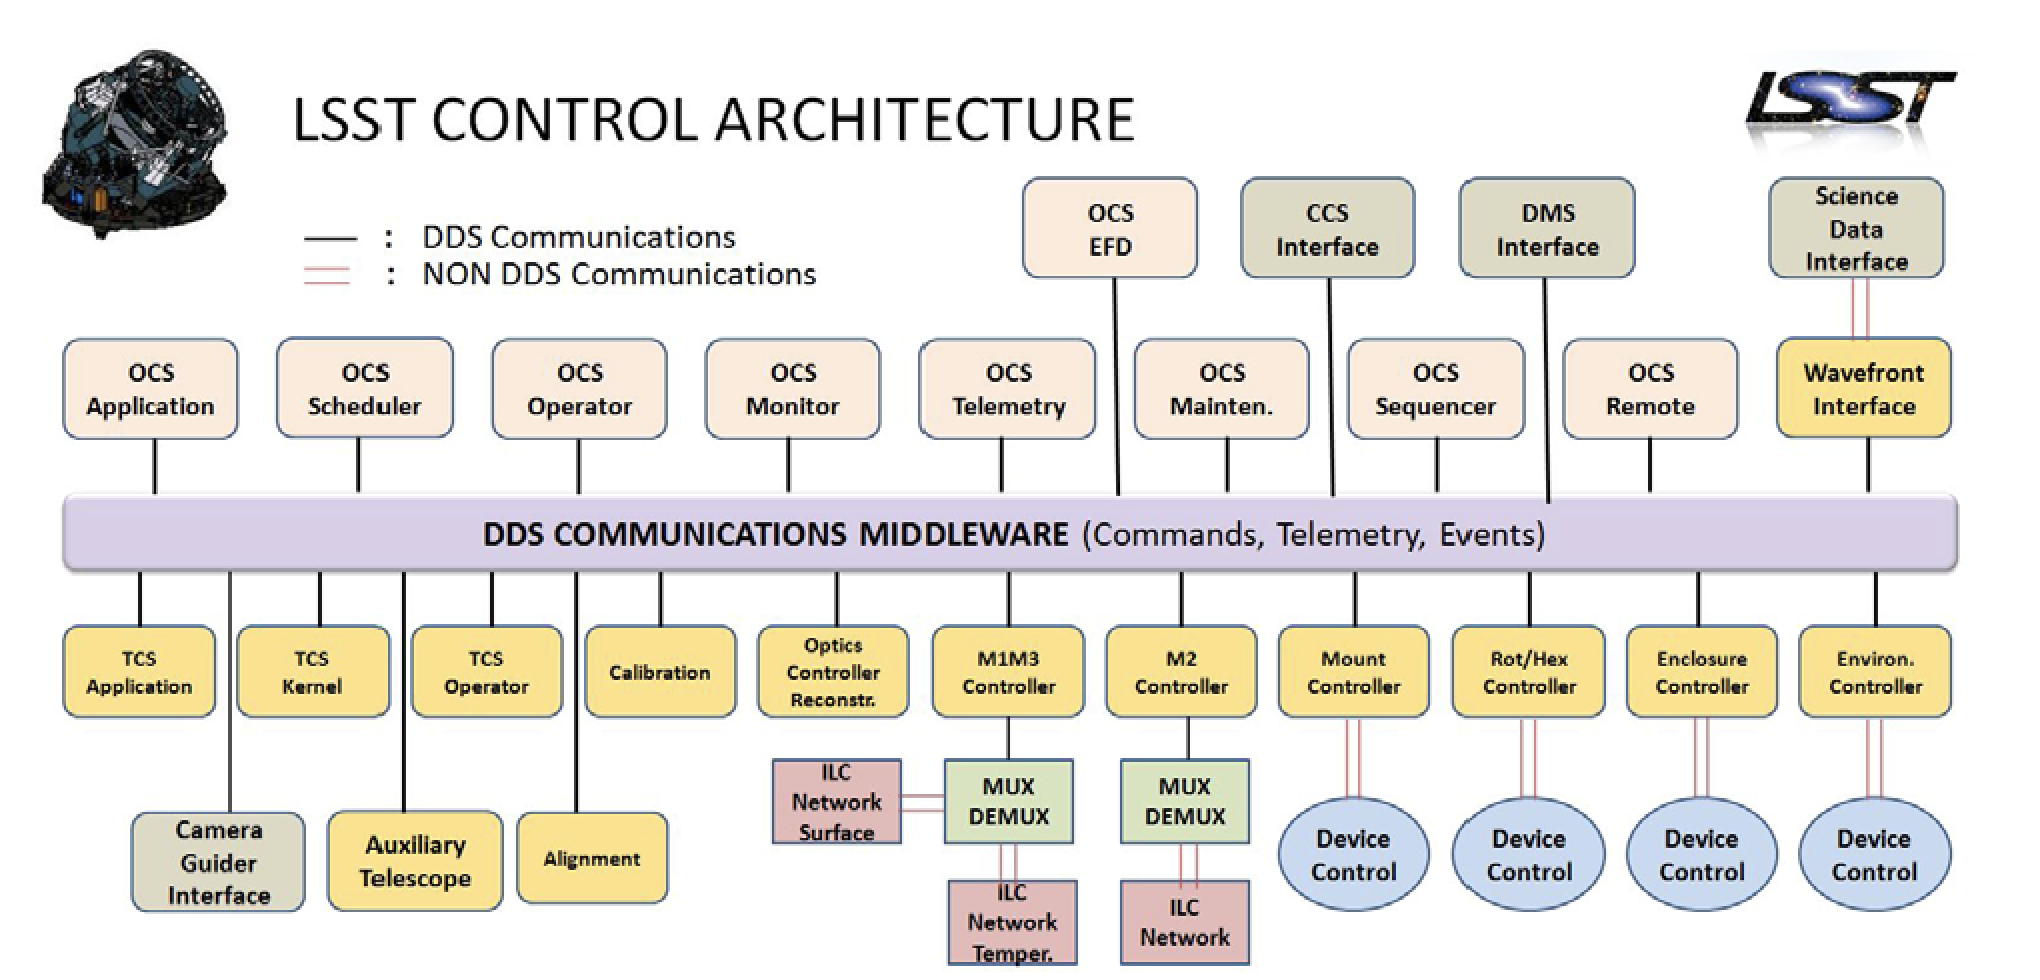
\includegraphics[width=0.8\textwidth]{arc}
\caption{High Level Architecture Diagram\label{fig:arc}}
\end{center}
\end{figure}

Broadly this may be seen as comprising:
\begin{itemize}
\item Infrastructure and Middleware :
	\begin{itemize}
	\item Service Access Layer (SAL) based on DDS
	\item Engineering and Facility Database (EFD)
	\item Operator Interface (based on LOVE)
	\item Script Queue  \footnote{\url{https://github.com/lsst-ts/ts_scriptqueue}}
	\item Python Scripting based on SalObj\footnote{\url{https://github.com/lsst-ts/ts_salobj}}
	\end{itemize}
\item The Scheduler \footnote{\url{https://github.com/lsst-ts/ts_scheduler}}
\item Potentially an Auxiliary and Main Telescope Control System (ATCS and TCS)\footnote {The precise nature and need for these is unclear now so they have lower priority.}
\item Controllable SAL Components (CSCs) - every device and some pseudo devices, including the scheduler, are CSCs. Some are coordinating other CSCs, the full hierarchy is shown for AuxTel in \figref{fig:atcscs} and the Main Telescope in \figref{fig:mtcscs}
\end{itemize}

\begin{figure}
\begin{center}
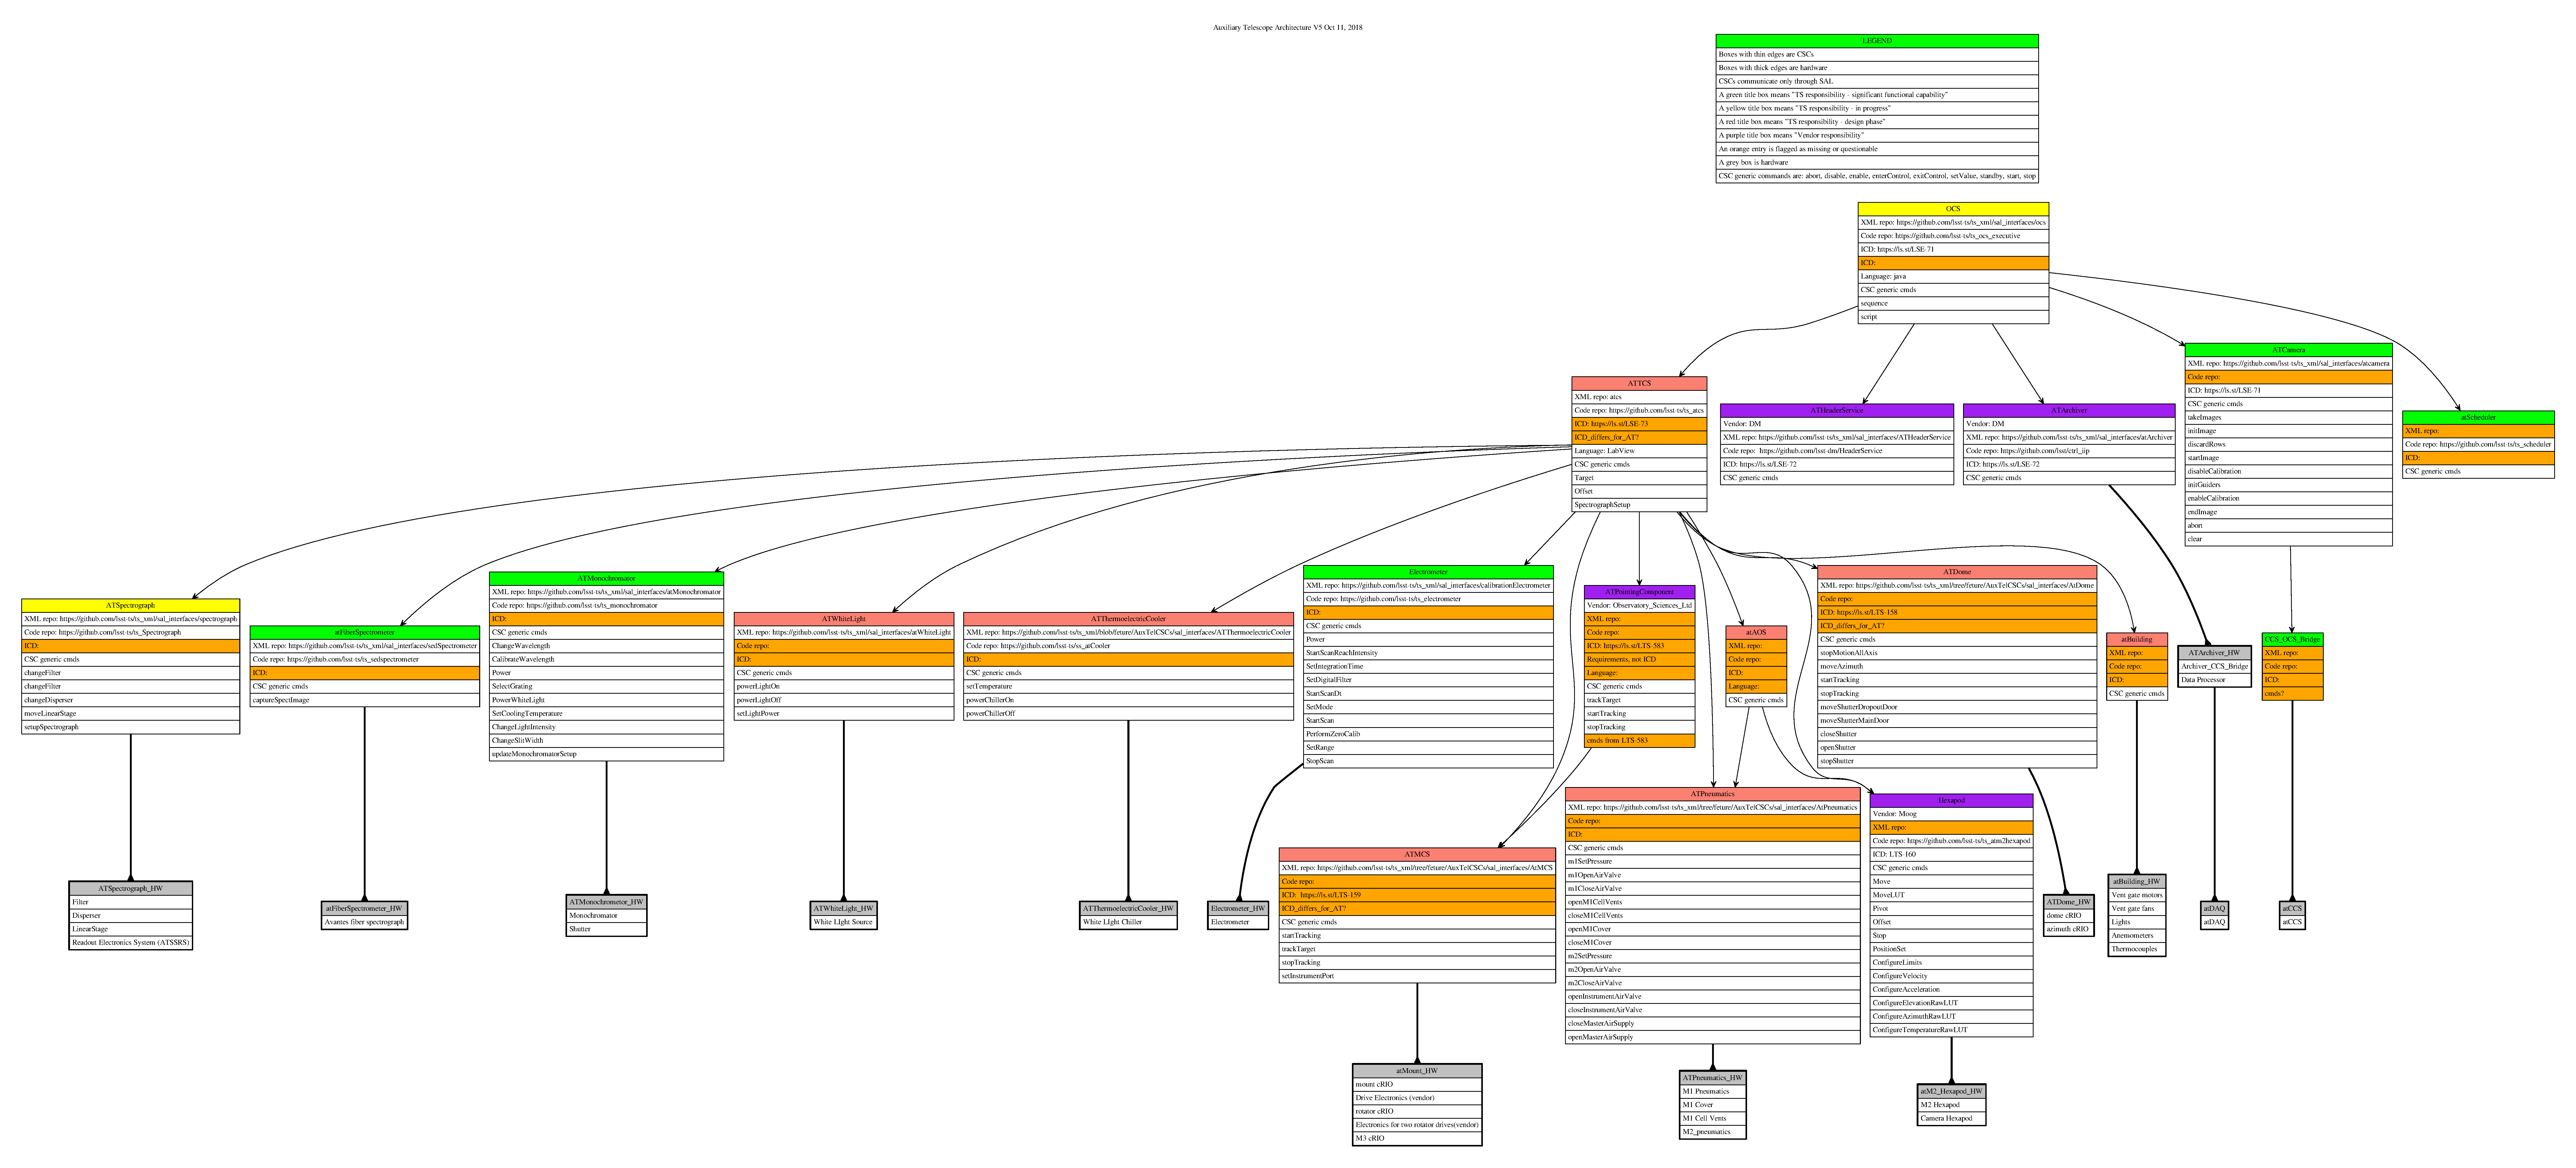
\includegraphics[width=0.9\textwidth]{AT}
\caption{Complete set of AuxTel CSCs\label{fig:atcscs}}
\end{center}
\end{figure}

\begin{figure}
\begin{center}
\includegraphics[width=0.9\textwidth]{LSST}
\caption{Complete set of Main Telescope CSCs\label{fig:mtcscs}}
\end{center}
\end{figure}

\subsection{Python and scripting }\label{sect:python}
The SalObj Python library provides a handy way of creating Controllable SAL Components (CSCs) which are not time critical. It also provides the basis for attaching to and scripting any orchestration of CSCs. A high level diagram is provided in \figref{fig:salobj}.

\begin{figure}
\begin{center}
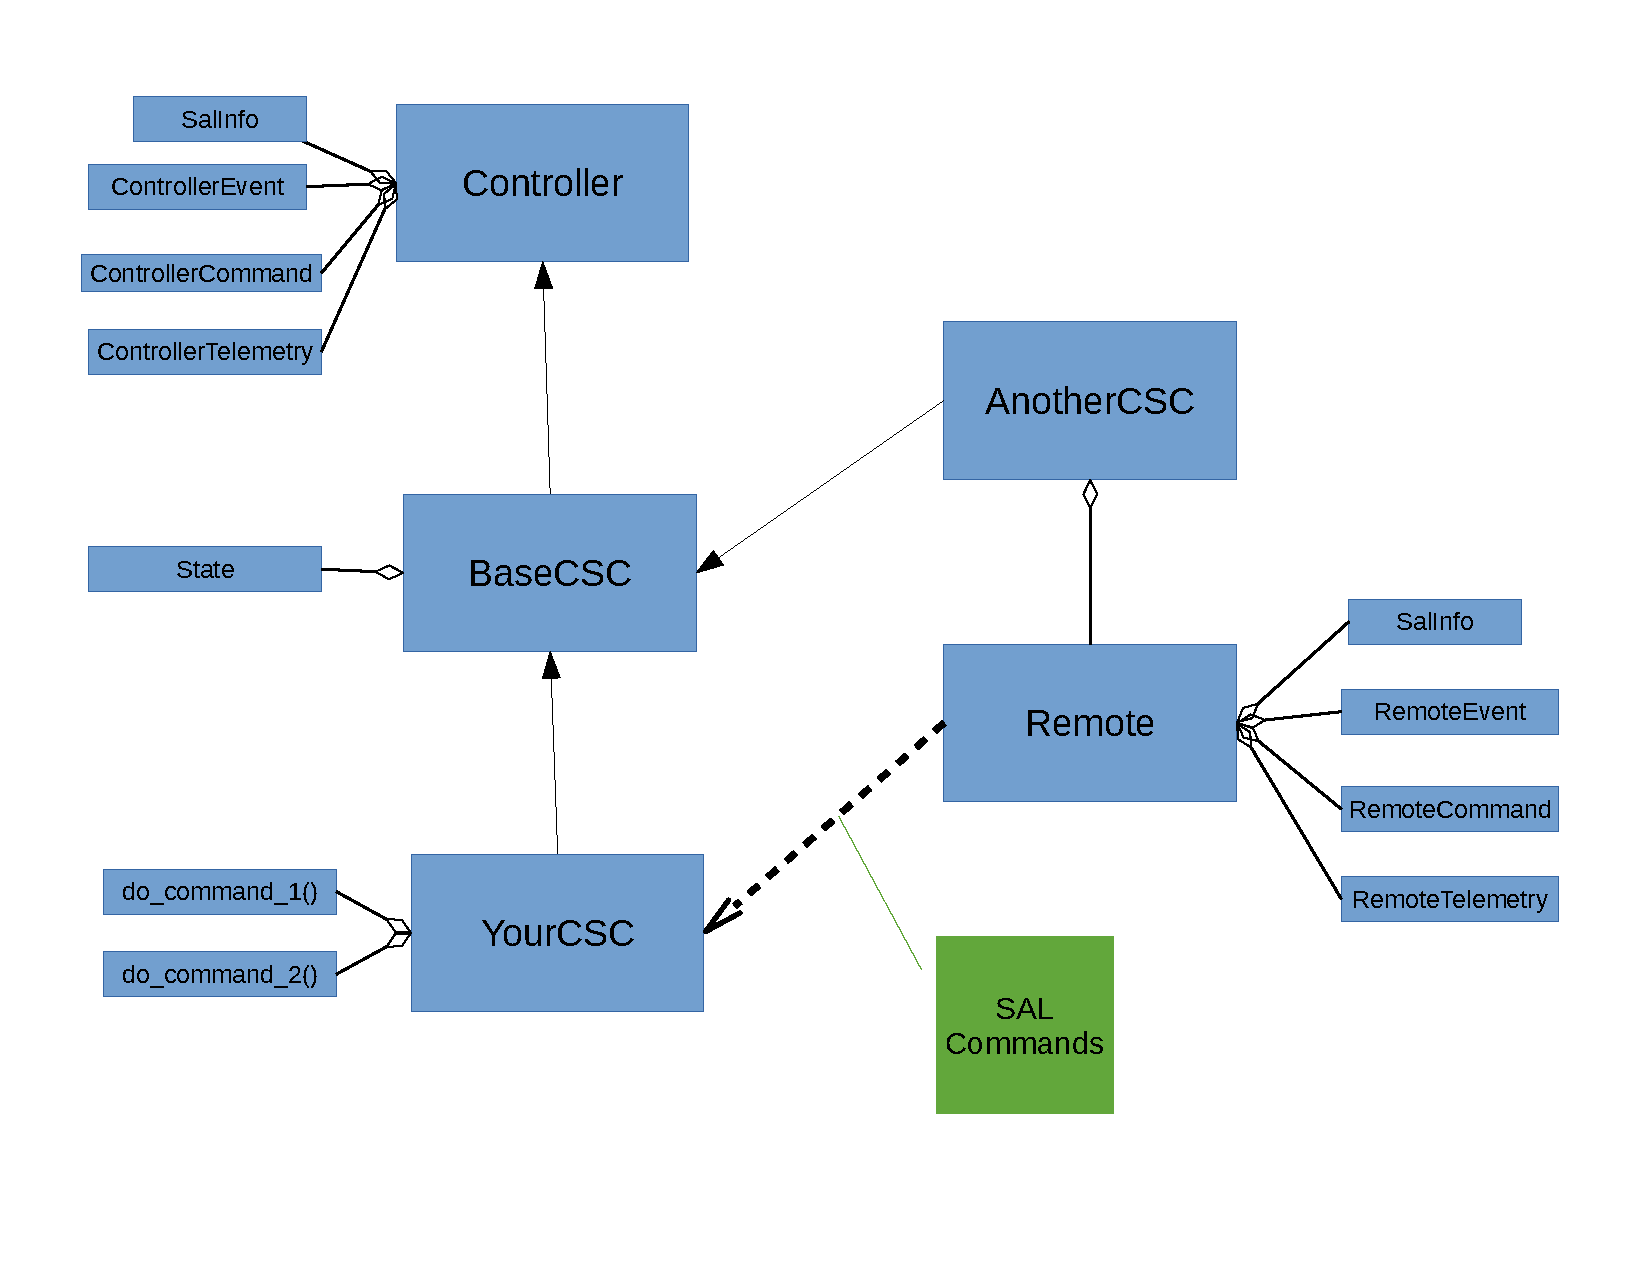
\includegraphics[width=0.9\textwidth]{SalobjClassDiag2}
\caption{SalObj python scheme for  CSCs\label{fig:salobj}}
\end{center}
\end{figure}

